\chapter{Sistemas Dinámicos Planos}
\label{cap:sistemasplanosautonomos}

\section{Conceptos Básicos} \label{sec:conceptosbasicos}

\begin{definition}[Sistema Dinámico Plano] \label{def:dynamicalsystem}
Sean $T \subseteq \R$ un semigrupo aditivo, $X$ un subconjunto de $\R^2$ y $\phi: T \times X \to X: (t,x) \mapsto \phi^t(x)$ una función. Un \emph{sistema dinámico plano} es una tupla $(T, X, \phi)$ que satisface las propiedades

\begin{enumerate}[(1)]
    \item $\phi \left( 0, x \right) = \phi \left( x \right)$ para todo $x \in
    X$. Equivalentemente $\phi^0 \equiv \text{id}_X$.
    
    \item $\phi \left( t, \phi \left( s, x \right) \right) = \phi \left(
    s + t, x \right)$ para todo $x \in X$ y $s, t \in T$. Equivalentemente $\phi^{s} \circ \phi^{t} \equiv \phi^{s + t}$.
\end{enumerate}

El conjunto $T$ se llama \emph{espacio de tiempos}, $X$ es llamado {\emph{espacio de estados (o de fase)}} y $\phi$ se conoce como {\emph{operador de evoluci\'on}}.
\end{definition}

Se puede pensar en un operador de evolución $\phi$ como una colección de funciones $\{ \phi^t: X \to X \}_t$, llamada también \emph{flujo}, que ``mueve'' un punto $x_0$ por el estado de fases $X$ a través de la curva $t \mapsto \phi^t(x_0)$ como en la figura \ref{fig:evolutionoperator}.

\begin{remark}
Un sistema dinámico se dice \emph{discreto} si el espacio de tiempos $T$ es discreto ($T \subseteq \Z$). En caso contrario, se dice \emph{continuo}.
\end{remark}

\begin{remark}
A menudo el operador de evolución $\phi$ no está definido en todo $T \times X$ sino en un subconjunto $U \subseteq T \times X$. En tal caso pedimos que $\{ 0 \} \times X \subseteq U$ y que las propiedades (1) y (2) de la definición \ref{def:dynamicalsystem} se satisfagan siempre que $(t, x)$ esté en $U$.

Es decir, dado $x \in X$ existe un subconjunto de tiempo (usualmente un intervalo) $I_x := \{ t \in T : (t,x) \in U \} \subseteq T$ tal que $\phi(t,x)$ está definida para todo $t \in I_x$.
\end{remark}

\begin{figure}[!ht] \centering
    \includegraphics[scale=1.3]{figures/evolution-operator.pdf}
    \caption{Operador de evolución.}
	\label{fig:evolutionoperator}
\end{figure}

En lo que sigue supondremos que $( T, X, \phi )$ es un sistema
dinámico.

Dado un $x_0 \in X$, un estado inicial, deseamos estudiar la geometr\'{\i}a del
conjunto de todos los posibles estados futuros y pasados del sistema
din\'amico, obtenidos a partir de $x_0$ haciendo uso del operador de
evoluci\'on $\phi$.
Para tal fin introducimos el concepto de órbita.

\begin{definition}
  \label{def:orbit}La {\emph{\'orbita (o trayectoria) positiva
  $\gamma^+_{x_0}$}}, {\emph{\'orbita negativa $\gamma^-_{x_0}$}} y
  {\emph{\'orbita $\gamma_{x_0}$}} de $x_0$ (o a trav\'es de $x_0$) son
  los subconjuntos del espacio de estados $X$, definidos por
  \[ \gamma^+_{x_0} := \left\{ \phi \left( t, x \right) : t \in I_{x_0},
     t \geq 0 \right\} = \left\{ \phi^t \left( x_0 \right) \right\}_{t
     \in I_{x_0}, t \geq 0}, \]
  \[ \gamma^-_{x_0} := \left\{ \phi^t \left( x_0 \right) \right\}_{t \in
     I_{x_0}, t \leq 0}, \]
  \[ \gamma_{x_0} := \gamma_{x_0}^+ \cup \gamma_{x_0}^- = \left\{ \phi
     \left( t, x \right) : t \in I_{x_0} \right\} = \left\{ \phi^t \left( x_0
     \right) \right\}_{t \in I_{x_0}} . \]
  Una \'orbita que consiste de un solo punto se llama {\emph{\'orbita
  constante}}.
\end{definition}

Mientras que las \'orbitas de un sistema din\'amico continuo son curvas en el
espacio $M$ parametrizadas por $t$ y orientadas en la direcci\'on de
crecimiento, las de un sistema din\'amico discreto son sucesiones de puntos
$\ldots ., f^{- 1} \left( x_0 \right), x_0, f \left( x_0 \right), f^2 \left(
x_0 \right), \ldots$ indizadas por enteros, como en la figura \ref{fig:orbits}.

\begin{figure}[ht] \centering
    \includegraphics[scale=1.3]{figures/orbits-continuousanddiscrete.pdf}
    \caption{Órbitas en un sistema dinámico continuo y uno discreto.}
	\label{fig:orbits}
\end{figure}

\begin{definition}
  \label{def:equilibrium}Un punto $x \in X$ es un {\emph{equilibrio}} (o
  {\emph{punto fijo o punto crítico}}) si $\gamma_x = \left\{ x \right\}$ (es decir,
  $\phi^t \left( x \right) = x$ para todo $t \in T$).
\end{definition}

Lo anterior implica que un sistema din\'amico puesto en un equilibrio permanece all\'{\i} por siempre. Rec\'{\i}procamente, las \'orbitas constantes corresponden a equilibrios del sistema.

\begin{definition}
  \label{def:periodicorbit}Una {\emph{\'orbita peri\'odica (o ciclo) $O$}}
  es una \'orbita no constante para la cual existe $t_0 \in T$ tal que
  $\phi^{t + t_0} \left( x_0 \right) = \phi^t \left( x_0 \right)$ para todo $t
  \in T$ y $x_0 \in O$.
  
  El m\'{\i}nimo $t_0$ que satisface lo anterior se llama
  {\emph{per\'{\i}odo de la \'orbita.}}
\end{definition}

Esto es, si el sistema din\'amico evoluciona desde un $x_0$ en un ciclo $O$,
regresar\'a exactamente a este punto $x_0$ a las $t_0$ unidades de tiempo. Por
tanto, una \'orbita peri\'odica de un sistema continuo es una curva
{\emph{cerrada}} en el espacio de fase.

\begin{figure}[!hb] \centering
    \includegraphics[scale=1.3]{figures/orbit-cycle.pdf}
    \caption{Una órbita periódica (ciclo) $O$ a través de $x_0$.}
	\label{fig:cycle}
\end{figure}

\begin{definition}[Diagrama de Fase]
  \label{def:phasediagram}Al dibujar la colecci\'on de todas las \'orbitas
  (con sus direcciones) obtenemos un {\emph{diagrama de fase}}.
\end{definition}
En la pr\'actica, solo unas \'orbitas representativas son consideradas en el diagrama de fase.

\begin{example}[Mapa Logístico]
Aunque se trata de un sistema unidimensional ($X \subseteq \R$) este es un buen ejemplo introductorio a la temática de sistemas dinámicos.

El mapa logístico es una relación de recurrencia no lineal popularizada por Robert May \cite{may76} como modelo demográfico de tiempo discreto.
Supongamos que existe un número máximo posible para los individuos de cierta población y sea $x_n \in [0,1]$ la fracción de dicho máximo de individuos que hay en el año $n$ en la población. Si $r$ es la tasa combinada de reproducción y mortandad de la población, el mapa logístico corresponde a la expresión

\begin{equation} \label{eq:mapalogistico}
x_{n+1} = rx_n(1-x_n).
\end{equation}

La ecuación \ref{eq:mapalogistico} está relacionada con dos fenómenos demográficos: el crecimiento es proporcional a la población existente $x_n$ cuando dicha población es pequeña. Existe, sin embargo, un valor crítico para el cual la tasa de mortalidad supera a la de crecimiento.
Esto pues $x_n^2$ es pequeño en comparación a $x_n$ cuando $x_n$ es pequeño pero este comportamiento se reversa una vez $x_n > 1$.

El mapa logístico puede entenderse como un sistema dinámico discreto con espacio de tiempo $T = \Z$, espacio de fase $X = [0,1]$ y operador de evolución dado por

\begin{equation} \label{eq:evolucionmapalogistico}
	\phi(n + 1, x) = x_{n+1} = rx_n(1-x_n).
\end{equation}

El sistema tiene un punto de equilibrio trivial en $x = 0$ pues $\phi^n(0) = 0$ para todo $n \in \Z$. Hay otro punto de equilibrio en $x = (r-1)/r$ pues

$$ \phi^1((r-1)/r) = r \frac{r-1}{r} \left(1 - \frac{r-1}{r} \right) = (r-1) \left( \frac{r - r + 1}{r} \right) = \frac{r-1}{r}. $$

El caso $r = 4$ es de particular interés pues presenta comportamiento caótico \cite[p.~19]{fractallectures} y porque la relación de recurrencia puede solucionarse de manera explícita \cite{lorenz64} como

$$  \phi^n(x) = \sin^2( 2^n \sin^{-1}( x^{1/2} ) ). $$

Algunas órbitas convergen al punto crítico $x = 0$ luego de un número finito de iteraciones pero la mayoría presentan un comportamiento errático. Por ejemplo, la órbita de $x = 1/2$ es $\gamma^+(1/2) = \{ 1/2, 1, 0, 0, 0, 0, ... \}$ mientras que las órbitas de $x = 0.6$ y $x = 0.61$, dos números muy cercanos, divergen en pocas iteraciones la una de la otra:

$$
	\begin{array}{lll}
		\gamma^+(0.6) & = & \{ 0.96, 0.1536, 0.5202816, 0.9983954912, 0.0064077373, ... \} \\
	\gamma^+(0.61) & = & \{ 0.9516, 0.18422976, 0.6011566221, 0.9590693512, 0.1570213231, ... \}.
	\end{array}
$$

\end{example}

\section{PVIs y Sistemas Autónomos}
\label{sec:propiedades_generales}

El principal interés de este documento es tratar sistemas planos continuos provenientes de ecuaciones diferenciales de segundo orden o, equivalentemente, de sistemas de dos ecuaciones diferenciales de primer orden.

En principio utilizamos la definición en \cite[p.~174]{dynandbif} y después de un importante teorema sobre existencia y unicidad indicamos cómo esta definición encaja con la de sistema dinámico plano (definición \ref{def:dynamicalsystem}).

\begin{definition}[Sistema Dinámico Plano Autónomo] \label{def:sistema_dinamico_plano}
Sea $I \subseteq \R$ un intervalo y $x_1,x_2:I \rightarrow \R$ funciones de clase $C^1$ en la variable $t$, a la que nos referiremos generalmente como el \textit{tiempo}.
Sean también $$f_i : \R^2 \rightarrow \R: (x_1, x_2) \rightarrow f_i(x_1, x_2); \hspace{0.5in} i \in \{1,2\}$$ funciones en dos variables.

Llamamos \emph{sistema dinámico plano autónomo} al par de ecuaciones diferenciales simultáneas de la forma

\begin{equation} \label{eq:sistema_dinamico_plano_v0}
\left\{
    \begin{array}{l}
        \dot{x_1} = f_1(x_1, x_2) \\
        \dot{x_2} = f_2(x_1, x_2)
    \end{array} \right.
\end{equation}
\end{definition}

\begin{remark}
Si utilizamos notación vectorial, podemos escribir $x = (x_1, x_2)$, $\dot{x} = (\dot{x_1}, \dot{x_2})$ y $f = (f_1, f_2)$, de modo que la ecuación \ref{eq:sistema_dinamico_plano_v0} obtiene ahora la forma más compacta

\begin{equation} \label{eq:sistema_dinamico_plano}
    \dot{x} = f(x)
\end{equation}
\end{remark}

Una \emph{solución} de la ecuación anterior está constituída, entonces, por un par de funciones diferenciables $x_1(t)$ y $x_2(t)$ (o equivalentemente, una función vectorial $x(t)$) tal que $x_1'(t) = f_1(x_1(t), x_2(t))$ y $x_2'(t) = f_2(x_1(t), x_2(t))$ para todo $t \in I$ (o equivalentemente $\dot{x} = f(x(t))$ para $t \in I$).

Nótese que la gráfica de cualquier solución de \ref{eq:sistema_dinamico_plano} es una curva en el espacio tridimensional $(t,x)=(t,x_1,x_2)$ que identificamos con un subconjunto de $\R^3$.

\begin{definition}[Problema de Valor Inicial]\label{def:pvi}
Un \emph{problema de valor inicial} para el sistema \ref{eq:sistema_dinamico_plano} es un problema de la forma

\begin{equation} \label{eq:pvi}
 \dot{x} = f(x); \hspace{0.5in} x(t_0) = x^0.
\end{equation}

\end{definition}

Como la función $f$ no depende explícitamente del tiempo $t$ (el sistema es autónomo), no hay pérdida de generalidad al suponer siempre que la condición inicial del problema de valor inicial \ref{eq:pvi} está especificada para $t_0 = 0$. Esta propiedad es conocida como la propiedad de \emph{traslación}.

\begin{lemma}[Propiedad de traslación] Supongamos que $x(t)$ es una solución de la ecuación \ref{eq:sistema_dinamico_plano} en un intervalo $I$, entonces $x(t-t_0)$ es también una solución.
\begin{proof}Hacemos $\tau = t - t_0$ y como $t$ no ocurre explícitamente en $f(x)$ entonces el lado derecho de la ecuación no cambia sino por reemplazar $t$ por $\tau$. De esta manera, $\phi(\tau)$ es solución de la ecuación transformada.
\end{proof}
\end{lemma}

Aunque las soluciones trasladadas $x(t)$ y $x(t-t_0)$ son diferentes corresponden a las mismas curvas en el diagrama de fase, como veremos más adelante.

Ahora, con el fin de estudiar un sistema dinámico plano como \ref{eq:sistema_dinamico_plano} es necesario garantizar la existencia de la solución $x(t)$ y, más aún, su unicidad de manera que no haya ambigüedad al tratar de definir un operador de evolución como se explicó en la sección anterior.

Como veremos a continuación, la continuidad de $f$ no es suficiente para ello.

\begin{example}Considérese el problema de valor inicial
    
$$
\left\{
    \begin{array}{l}
        \dot{x} = (\dot{x_1}, \dot{x_2}) = (\sqrt{x_1}, 0), \\
        x(0) = 0.
    \end{array}
\right.
$$

Es claro que la ecuación diferencial tiene infinidad de soluciones, pero aún el PVI, con la condición prescrita $x(0) = 0$ carece de solución única. Es fácil verificar que $x(t) \equiv 0$ y $y(t) = (\frac{t^2}{4}, 0) $ son ambas soluciones del PVI.
\end{example}

El siguiente teorema, que es una generalización a dos dimensiones de un resultado clásico del análisis de ecuaciones diferenciales de primer orden, demuestra que esta dificultad puede resolverse suponiendo que $f$ es de clase por lo menos $C^1$.

\begin{theorem}[Existencia y Unicidad] \label{teo:existenciayunicidad} Supongamos que $f$ es una función continua localmente Lipschitz definida en $\R^2$. Entonces para cualquier $x^0 \in \R^2$ existe un intervalo (posiblemente infinito) $I_{x^0} \equiv (\alpha_{x^0}, \beta_{x^0})$ que contiene a $t_0 = 0$ y una \emph{única} solución $\phi(t,x^0)$ del problema de valor inicial \ref{def:pvi} definida para todo $t \in I_{x^0}$ que satisface la condición $\phi(0, x^0) = x^0$ y es, además, de clase $C^1$.
\begin{proof}
Ver \cite[p.~10]{barrvalls} o \cite[p.~163]{smale}.
\end{proof}
\end{theorem}

Justificamos ahora el uso del nombre ``sistema dinámico'' al tratar un sistema de ecuaciones diferenciales como el de la ecuación \ref{eq:sistema_dinamico_plano_v0}.

\begin{proposition}Si $f$ es localmente Lipschitz entonces el sistema dinámico autónomo plano $\dot{x} = f(x)$ (definición \ref{def:sistema_dinamico_plano}) es un sistema dinámico (definición \ref{def:dynamicalsystem}).
\begin{proof}

Por teorema \ref{teo:existenciayunicidad} sabemos que existe una solución $x(t,x^0)$ tal que $x(0,x^0) = x^0$. En particular, la propiedad (2) de la definición \ref{def:dynamicalsystem} se satisface trivialmente.

Debemos demostrar que $\phi^t(x^0) = x(t,x^0)$ constituye un flujo (operador de evolución) como en la definición \ref{def:dynamicalsystem}. Esto es, satisface la propiedad (2).

Sea $s \in \R$ y consideremos la función $y: \R \to \R^2$ definida por 

$$ y(t) = x(t+s, x^0).$$

Claramente $y(0) = x(s,x^0)$ y además

$$ y'(t) = x'(t+s,x^0) = f(x(t+s, x^0)) = f(y(t))  $$

para $t \in \R$. En particular, $y$ también es una solución del PVI entonces por unicidad debe tenerse

$$ x(t+s,x^0) = y(t) = x(t, y(0)) = x(t, x(s,x^0))$$

que es precisamente la propiedad (2).
\end{proof}
\end{proposition}

Entramos en materia, introduciendo el oscilador armónico lineal, que será utilizado en adelante.

\begin{example}[Oscilador armónico lineal] \label{ex:osciladorarmonico} Considérese la ecuación de segundo orden $\ddot{y} + y = 0$ que puede transformarse en el par de ecuaciones de primer orden

\begin{equation} \label{eq:osciladorarmonico}
	\begin{array}{l}
		\dot{x_1} = x_2 \\
		\dot{x_2} = -x_1.
	\end{array}
\end{equation}

El teorema \ref{teo:existenciayunicidad} garantiza la existencia de las soluciones de este sistema para cualquier valor prescrito en $t_0 = 0$. Por ejemplo, para $x^0 = (x_1^0,x_2^0) = (0,1)$ la solución del sistema es $x_1(t) = \sin(t)$ y $x_2(t) = \cos(t)$.
\end{example}

La figura \ref{fig:osciladorarmonico} (a) ilustra la gráfica de la solución del oscilador armónico en el espacio tridimensional $(t,x_1,x_2)$ tal que pasa por $(0,1)$ en $t_0 = 0$. Las componentes $x_1(t), x_2(t)$ de la solución aparecen también en la figura \ref{fig:osciladorarmonico} (c).

En general, a la curva solución $x(t)$ tal que $x(0) = x^0$ se le llamará \emph{trayectoria} a través de $x^0$.

Como el sistema es autónomo (la función $f$ es independiente de $t$) resulta natural considerar las proyecciones de las trayectorias sobre el plano $x_1x_2$ a las que llamaremos \emph{órbitas}. Una órbita típica del oscilador armónico aparece en la figura \ref{fig:osciladorarmonico} (b).

\begin{figure}
\centering
    \includegraphics[scale=1.0]{figures/osciladorarmonico-solucion.pdf}\\(a) \\
    \includegraphics[scale=1.0]{figures/osciladorarmonico-orbita.pdf}\\(b) \\ 
    \includegraphics[scale=1.0]{figures/osciladorarmonico-soluciones.pdf}\\(c) \\
    \caption{Oscilador armónico lineal: (a) trayectoria a través de $(0,1)$, (b) órbita circular que resulta de proyectar la trayectoria en el plano $x_1x_2$ y campo de direcciones, (c) gráficas de las soluciones $x_1(t), x_2(t)$ vs $t$.}
	\label{fig:osciladorarmonico}
\end{figure}

Ahora, aún cuando contamos con el teorema \ref{teo:existenciayunicidad} para asegurarnos de que existen funciones $x_1(t), x_2(t)$ que satisfacen el sistema, resulta, en general, muy complicado hallar fórmulas cerradas explícitas para tales funciones. Por este motivo es de suma importancia y es el objetivo principal de este documento, el estudio cualitativo de las soluciones (su comportamiento) aún sin tener acceso a las mismas de antemano.

La independencia de $t$ nos permite iniciar este estudio a través de lo que llamaremos \emph{campo de direcciones}: si consideramos cualquier solución $(x_1(t),x_2(t))$ de \ref{eq:sistema_dinamico_plano} como la posición en el plano de una partícula en el instante $t$, entonces el par de ecuaciones $\dot{x_1} = f_1(x_1,x_2)$ y $\dot{x_2} = f_2(x_1,x_2)$ implican que $(\dot{x_1}(t),\dot{x_2}(t))$ es el vector tangente al punto $(x_1,x_2)$; es decir, puede entenderse como la velocidad de la partícula en ese instante. Así pues, el campo vectorial definido por 

$$ V(x_1,x_2) = (\dot{x_1}, \dot{x_2})$$

nos permite describir el comportamiento aproximado de la trayectoria de la partícula (esto es, una solución del sistema) para cualquiera condiciones iniciales aún sin conocer las funciones $x_1(t)$ o $x_2(t)$.

\begin{example} \label{ej:sistemahiperbolas}
Volvemos al oscilador armónico \ref{ex:osciladorarmonico}, cuyo campo de direcciones aparece en la figura \ref{fig:osciladorarmonico} (c).
Al observar el campo no resulta difícil imaginar que todas las órbitas deben ser círculos con centro en $(0,0)$. Esto puede formalizarse a partir del estudio de su campo vectorial:

$$ V(x_1,x_2) = (x_2, -x_1). $$

Empezamos por notar que si $V(x_1,x_2) = (0,0)$ entonces $x_1 = x_2 = 0$ y estamos hablando de la solución $x(t) = 0$ que satisface la condición inicial $x^0 = 0$. Si en cambio $(x_1(t),x_2(t))$ es cualquier otra solución a través de $x^0 \neq 0$ entonces debe cumplirse que 

$$
\begin{array}{ccl}
	\dfrac{d}{dt} || (x_1(t),x_2(t))  ||^2 & = & 2x_1(t)\dot{x_1}(t) + 2x_2(t)\dot{x_2}(t) \\
									   & = & 2x_1(t)x_2(t) - 2x_2(t)x_1(t) \\
									   & = & 0.
\end{array}
$$

Y por lo tanto para todo $t$ se tiene

$$ ||(x_1(t), x_2(t))||^2 = ||x^0||^2. $$

Es decir, la solución está en el círculo de radio $||x^0||$ centrado en el origen, como se quería verificar.
\end{example}

\begin{figure}[h] \centering
    \includegraphics[scale=0.5]{figures/osciladorarmonico-diagramafase.png}
    \caption{$\clubsuit$ Diagrama de fase del oscilador armónico lineal.}
\end{figure}

\begin{example}
Haremos un análisis similar al del ejemplo anterior para la ecuación de segundo orden $$ \ddot{y} - y = 0$$ que puede transformarse en el sistema de ecuaciones de primer orden:

$$
\begin{array}{l}
	\dot{x_1} = x_2 \\
	\dot{x_2} = x_1
\end{array}
$$

Notamos que las órbitas en el plano de fase satisfacen

$$ \dfrac{dx_2}{dx_1} = \frac{x_1}{x_2}. $$

Integrando produce la familia de hipérbolas

$$ x^2 - y^2 = c $$

donde $c$ es una constante.

En particular, cuando $c = 0$ obtenemos la solución constante $x = y = 0$ correspondiente a la órbita de $(0,0)$. Todas las demás órbitas son no constantes.

\begin{figure}[!ht] \centering
	\includegraphics[scale=0.5]{figures/linearsystem-hyperbolas.png}
	\caption{$\clubsuit$ Diagrama de fase para la ecuación de segundo orden $\ddot{x} - x = 0$.}
\end{figure}

\end{example}

\section{Clasificación de las soluciones}

Por el teorema \ref{teo:existenciayunicidad} una solución del sistema autónomo plano $\dot{x} = f(x)$ que satisface $x(0) = x^0$ es única. 

A continuación consideramos tres tipos básicos para tales soluciones.

\subsection{Puntos Críticos}

\begin{definition}[Punto Crítico] Una solución constante $x(t) = x^0$ se llama \emph{punto crítico}, \emph{solución de equilibrio} o también \emph{punto (solución) estacionario}.
\end{definition}

Como todo punto crítico $\bar{x} = (x_1,x_2)$ satisface $\dot{\bar{x}} = 0$ entonces puede hallarse resolviendo $f(x) = 0$. Es decir, el par de ecuaciones algebraicas
$$ f_1(x_1, x_2) = 0, \hspace{0.2in} f_2(x_1, x_2) = 0.$$

Por supuesto, las órbitas en el plano de fase correspondientes a soluciones de equilibrio son órbitas constantes (constan de un sólo punto).

En el capítulo siguiente se estudiará el comportamiento de todas las soluciones de un sistema lineal (y más adelante no lineal), lo que nos permitirá hacer una clasificación aún más completa de los puntos de equilibrio. Por ahora, los catalogamos en estables o inestables según sea el comportamiento de soluciones (órbitas) ``cercanas'' a la de equilibrio.

\begin{definition}[Punto crítico estable]Un punto crítico $\bar{x}$ se dice \emph{estable} si dado $\epsilon > 0$ existe un $\delta > 0$ tal que para cualquier solución $x = x(t)$ del sistema tal que $|| x(0) - \bar{x} || < \delta$ se cumple que
$$ || x(t) - \bar{x} || < \epsilon$$
para todo $t \geq 0$.

Un punto que no es estable se dice \emph{inestable}.
\end{definition}

Intuitivamente, una solución de equilibrio es estable si toda solución (órbita) que comienza suficientemente cerca de la misma permanece cerca todo el tiempo.

\begin{definition}[Punto crítico asintóticamente estable]Un punto crítico $\bar{x}$ se dice \emph{asintóticamente estable} si es estable y existe $\delta > 0$ tal que para toda solución $x = x(t)$ del sistema tal que $|| x(0) - \bar{x} || < \delta$ se tiene $$\lim_{t \to \infty} x(t) = \bar{x}. $$
\end{definition}

Lo anterior implica que la trayectoria de toda solución que comience suficientemente cerca de un punto asintóticamente estable no sólo debe permanecer cerca sino que a la larga converge al equilibrio $\bar{x}$. Debido al teorema de existencia y unicidad \ref{teo:existenciayunicidad}, estas trayectorias no pueden llegar a $\bar{x}$ en un tiempo finito.

\begin{figure}[!ht] \centering
	\includegraphics[scale=1.0]{figures/equilibrium-stable.pdf}\\(a) \\
	\includegraphics[scale=1.0]{figures/equilibrium-asymptoticallystable.pdf}\\(b) \\
	\caption{(a) Equilibrio estable. (b) Equilibrio asintóticamente estable.}
\end{figure}

\begin{example}
La única solución de equilibrio del oscilador armónico (ejemplo \ref{ex:osciladorarmonico}) y el sistema plano del ejemplo \ref{ej:sistemahiperbolas} es $\bar{x} = \bar{x}(t) = 0$.

El equilibrio del oscilador armónico es un ejemplo de un equilibrio estable que no es asintóticamente estable pues dado $\epsilon > 0$ todas las soluciones en el disco $D := D(0, \delta)$ permanecen dentro del disco $D$ para cualquier $0 < \delta \leq \epsilon$. Sin embargo, toda órbita es periódica distinta de $\gamma(0)$ y no tiende a $0$.

El equilibrio del sistema del ejemplo \ref{ej:sistemahiperbolas} es inestable. Sin embargo, el sistema presenta un comportamiento interesante: hay toda una familia de soluciones $x(t)$ tales que $x(t) \to 0$ aún cuando el equilibrio no es asintóticamente estable.

\end{example}


\subsection{Soluciones Periódicas}

Ya nos hemos encontrado antes con soluciones periódicas de sistemas planos (por ejemplo, en el oscilador armónico \ref{eq:osciladorarmonico}). En esta sección formalizamos el concepto y probamos la equivalencia entre las órbitas cerradas (ciclos) en el espacio de fase y las soluciones periódicas.

\begin{definition}[Solución Periódica] Una solución $x = x(t)$ del sistema $\dot{x} = f(x)$ se dice \emph{periódica} si existe un $T > 0$ tal que $x(t+T) = x(t)$ para todo $t$. En tal caso, al mínimo valor de $T$ se le llama \textit{período} de la solución.
\end{definition}

En la definición no se admite el caso $T=0$, esto es, las soluciones constantes no están consideradas de manera explícita como periódicas.

Resulta evidente que toda solución periódica produce órbitas cerradas (ciclos) en el espacio de fase. Mostraremos a continuación que el recíproco también es cierto.

\begin{lemma}
Toda solución periódica de la ecuación autónoma \ref{eq:sistema_dinamico_plano} $\dot{x} = f(x)$ corresponde a un ciclo del espacio de fase y todo ciclo corresponde a una solución periódica.
\end{lemma}
\begin{proof}
La primera parte es trivial. Para la segunda parte, supongamos que $\gamma$ es una órbita cerrada (ciclo) en el espacio de fase y que $x^0 \in \gamma$.
Por el teorema \ref{teo:existenciayunicidad} hay una solución $x = x(t)$ tal que $x(0) = x^0$ cuya trayectoria es precisamente el ciclo $C$ y, por unicidad, no puede contener ningún punto crítico, de manera que $|| f(x) || \geq a > 0$ para todo $x \in C$.
Esto es equivalente a que $|| \dot{x} || \geq a > 0$ así que debe tenerse para algún $t = T$ que $x(T) = x^0$ de nuevo. Queremos probar que $T$ es el período de la solución, es decir, que $x(t+T) = x(t)$ para todo $t \in \R$. Para ello, considérese $t = nT + t_1$ donde $n \in \Z$ y $0 < t_1 < T$. Por la propiedad de traslación como $x(t)$ es una solución con $x(t_1) = x^1$ entonces $x(t - nT)$ es una solución con $x(t - nT) = x^1$. Es decir, $$ x(t_1) = x(t_1 + nT)$$ para todo $t_1$ tal que $0 < t_1 < T$.

Esto implica que $x$ es $T$-periódica.
\end{proof}

\subsection{Curvas Integrales}

En general, las demás soluciones de un sistema plano producen órbitas arbitrarias en el plano de fase que no se cruzan.
A menudo es posible integrar las ecuaciones de un sistema plano para obtener una familia de curvas integrales (soluciones) de manera implícita.

Supóngase que el sistema plano está dado, como en \ref{eq:sistema_dinamico_plano} por el par de ecuaciones

$$
\begin{array}{l}
	\dot{x_1} = f_1(x_1,x_2) \\
	\dot{x_2} = f_2(x_1,x_2)
\end{array}
$$

Entonces

\begin{equation} \label{eq:ecprimerordencurvaintegral}
	\dfrac{dx_2}{dx_1} = \frac{dx_2/dt}{dx_1/dt} = \frac{\dot{x_2}}{\dot{x_1}} = \dfrac{f_2(x_1,x_2)}{f_1(x_1,x_2)}.
\end{equation}

La ecuación \ref{eq:ecprimerordencurvaintegral} es una ecuación diferencial de primer orden para $x_1$ o $x_2$ y las órbitas de las soluciones del sistema plano corresponden a las curvas integrales de esta ecuación diferencial.

\begin{example}
Volvemos al oscilador armónico del ejemplo \ref{ex:osciladorarmonico} que corresponde al sistema:

$$
\begin{array}{l}
	\dot{x_1} = x_2 \\
	\dot{x_2} = -x_1
\end{array}
$$

En este caso la ecuación \ref{eq:ecprimerordencurvaintegral} es

$$ \dfrac{dx_2}{dx_1} = \frac{-x_1}{x_2}.$$

Si se separan las variables y se integra se encuentra que las soluciones deben satisfacer:

$$ \frac{1}{2}x_1^2 + \frac{1}{2}x_2^2 = c.$$

Es decir, el conjunto de curvas integrales es una familia de círculos centrados en el origen con radio $2c$ para $c \in \R^+$. El punto de equilibrio $x = 0$ se obtiene cuando $c = 0$.

Esto coincide con lo que ya habíamos visto antes.
\end{example}


\begin{figure}[!ht] \centering
	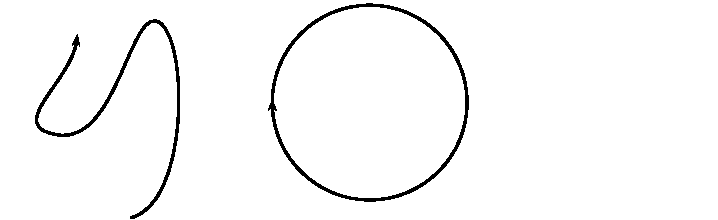
\includegraphics[scale=1.1]{figures/orbita-tipos.pdf}
	\caption{Una órbita arbitraria y un ciclo.}
\end{figure}

\section{Ejemplos Clásicos}

\begin{example}[Péndulo matemático] \label{ej:pendulo}

\begin{figure}[!hb] \centering
	\includegraphics[scale=1.0]{figures/pendulum.pdf}
	\caption{Ilustración del péndulo matemático.}
	\label{fig:pendulo}
\end{figure}

Supongamos que una masa $m$ se encuentra unida al extremo inferior de una varilla de longitud $l$. Sabemos que el arco $s$ de un círculo de radio $l$ se relaciona con el ángulo central $\theta$ mediante la fórmula $s = l\theta$, de manera que la aceleración angular está dada por

$$ a = \dfrac{d^2s}{dt^2} = l \dfrac{d^2\theta}{dt^2}.$$

En ausencia de fuerzas externas o amortiguamiento, la única fuerza que actúa sobre la masa es su peso $mg$, cuya componente tangencial es $-mg\sin\theta$, así que por la segunda ley de Newton:

$$ ml \dfrac{d^2\theta}{dt^2} = ma = -mg\sin\theta.$$

De donde se deduce la ecuación de segundo orden para $\theta$:

\begin{equation} \label{eq:pendulo0}
	\dfrac{d^2\theta}{dt^2} + \frac{g}{l}\sin\theta = 0.
\end{equation}

Dependiendo de la longitud $l$ de la varilla, la razón $g/l$ cambia, de manera que la ecuación \ref{eq:pendulo0} puede reescribirse como

\begin{equation} \label{eq:pendulo}
	\dfrac{d^2\theta}{dt^2} + \lambda\sin\theta = 0.
\end{equation}

A menudo se asumirá que $\lambda = 1$ al estudiar el péndulo matemático.

Sabemos que la ecuación \ref{eq:pendulo} puede reescribirse como un sistema plano haciendo $x_1 = \theta$ y $x_2 = \dot{\theta}$ obteniendo así:

\begin{equation}
	\begin{array}{l}
		\dot{x_1} = x_2 \\
		\dot{x_2} = -\lambda \sin\theta.
	\end{array}
\end{equation}

Debido a que el término $\sin\theta$ hace que la ecuación anterior sea no lineal, a veces se aproxima, para $\theta$ pequeño, $\sin(\theta) \approx \theta$, obteniéndose en lugar de \ref{eq:pendulo} la ecuación lineal

$$ \ddot{\theta} + \lambda\theta = 0,$$

conocida como oscilador armónico lineal y que ya se estudió en el ejemplo \ref{ex:osciladorarmonico}.


\begin{figure}[!ht] \centering
	\includegraphics[scale=0.5]{figures/pendulomatematico-fase.png}
	\caption{$\clubsuit$ Diagrama de fase del péndulo, con centros $(n\pi, 0)$ para $n \in \Z$.}
	\label{fig:pendulomatematico}
\end{figure}

\end{example}

\begin{example}[Modelo depredador-presa de Lotka-Volterra]\label{ex:lotkavolterra}

Consideremos dos poblaciones que interactúan entre sí: una especie de presa $x_1$ y su depredador, $x_2$. Un modelo matemático para la población de ambas especies es el modelo \emph{depredador-presa} de Lotka y Volterra, propuesto inicialmente por Alfred J. Lotka \cite{lotka10,lotka25,volterra} y que opera bajo las siguientes suposiciones:

\begin{enumerate}
	\item La población de presa $x_1$ no sufre de escasez de comida ni otros factores ambientales en su contra.
	\item La alimentación de la población depredadora $x_2$ depende exclusivamente del tamaño de la población presa $x_2$.
	\item La tasa de cambio de la población es proporcional a su tamaño.
\end{enumerate}

El sistema Lotka-Volterra corresponde entonces, al par de ecuaciones diferenciales
\begin{equation} \label{eq:lotkavolterra}
	\begin{array}{lll}
		\dot{x_1} & = & a_1x_1 - a_2x_1x_2 \\
		\dot{x_2} & = & -a_3x_2 + a_4x_1x_2,
	\end{array}
\end{equation}

donde $a_1, a_2, a_3$ y $a_4$ son constantes positivas.

Aunque el modelo es simple tiene sentido físico: en ausencia de interacción entre las especies ($a_2 = a_4 = 0$) el modelo se reduce a uno en el que la población presa $x_1$ crece sin límite, mientras que la población de depredadores $x_2$ se extingue eventualmente.
En cambio, cuando hay interacciones (que se consideran proporcionales al producto de las poblaciones $x_1x_2$) el crecimiento de $x_1$ se ve afectado mientras que la tasa de crecimiento de $x_2$ mejora, como es de esperarse.

Es fácil verificar que el sistema \ref{eq:lotkavolterra} tiene dos puntos críticos: a saber $(0,0)$ y $(a_3 / a_4, a_1 / a_2)$.
La estabilidad del primero de ellos puede tratarse mediante linealización (ver sección \ref{sec:linealizacion}) y resulta ser de punto de silla.

Sin embargo, el otro punto crítico es no hiperbólico de manera que debe hacerse un análisis distinto al de linealización. No es difícil concluir, en este caso, que se trata de un centro (ver sección \ref{subsec:centrooespiral}) y que los niveles de la población de presa y depredador oscilan alrededor de este punto fijo.

\begin{figure}[!ht] \centering
	\includegraphics[scale=0.5]{figures/lotkavolterra.png}
	\caption{$\clubsuit$ Diagrama de fase del modelo presa-depredador de Lotka-Volterra.}
	\label{fig:lotkavolterra}
\end{figure}

El modelo Lotka-Volterra no tiene en consideración la competencia entre las propias especies ya sea por la obtención de los recursos naturales (en el caso de la presa) o por el número limitado de presas (en el caso de los depredadores). Un sistema más realista que tiene presente estas interacciones se conoce como modelo de \emph{especies en competencia} (ver, por ejemplo, \cite[p.~171]{dynandbif}).

\end{example}

\newpage
\begin{example}[Oscilador de Van der Pol] \label{ex:vanderpol}

Además de los fenómenos biológicos, el estudio de los circuitos eléctricos también da origen a ecuaciones diferenciales importantes: el \emph{oscilador de Van der Pol} es un tipo de oscilador con amortiguamiento no lineal, planteado por el físico holandés Balthasar Van der Pol \cite{vanderpol} que obedece la ecuación diferencial de segundo orden

\begin{equation} \label{eq:vanderpol}
	\ddot{x} - \lambda (1-x^2)\dot{x} + x = 0.
\end{equation}

Aquí, $x$ es la posición (dependiente de $t$) y $\lambda$ es un parámetro que determina la no linealidad y el amortiguamiento.

La forma bidimensional de la ecuación \ref{eq:vanderpol} corresponde al sistema

\begin{equation} \label{eq:vanderpol2}
	\begin{array}{l}
		\dot{x_1} = x_2 \\
		\dot{x_2} = \lambda (1-x_1^2)x_2 - x_1.
	\end{array}	
\end{equation}

Cuando $\lambda = 0$ la ecuación \ref{eq:vanderpol} se reduce a la del oscilador armónico lineal. En cualquier otro caso ($\lambda > 0$) el sistema \ref{eq:vanderpol2} posee un ciclo límite (ver teorema \ref{teo:poincarebendixson}) y el punto crítico en el origen es inestable.

\begin{figure}[!ht] \centering
	\includegraphics[scale=0.45]{figures/vanderpol.png}
	\caption{$\clubsuit$ Diagrama de fase del oscilador de Van der Pol. Se evidencia el ciclo límite.}
	\label{fig:vanderpol}
\end{figure}

\end{example}
